\documentclass[11pt]{article}
\usepackage[latin1]{inputenc}
\usepackage{a4wide}
\usepackage{amsmath}
\usepackage{amsfonts}
\usepackage{amssymb}
\usepackage{graphicx}
\usepackage{enumerate}
\usepackage{epstopdf}
\usepackage{float}
\usepackage{multicol}
\usepackage{hyperref}
\epstopdfsetup{outdir=./images/}
\usepackage{subcaption}
\usepackage[table,xcdraw]{xcolor}

\renewcommand{\thesubsection}{(\alph{subsection})}
\newcommand{\floor}[1]{\lfloor #1 \rfloor}

\title{Natural Computing, Assignment 3}
\author{Dennis Verheijden - s4455770 \and Pauline Lauron - s1016609 \and Joost Besseling - s4796799}
\begin{document}
\maketitle

\section*{Combining, Bagging \& Random Forests}
\section{}
\subsection{}
\begin{itemize}
	\item 
	The probability that all three doctors give the correct answer is $ 0.8^3 = 0.512$. 
	\item 
	The probability that exactly 2 doctors make the right call is $0.8*0.8*0.2 + 0.8*0.2*0.8 + 0.2*0.8*0.8 = 0.384$. Therefore, the probability that \emph{at least} two doctors make the right call is $0.512 + 0.384 = 0.896$.
	\item  The probability that this group makes the right decision based on majority voting is $0.512 + 0.384 = 0.896$ since the majority is when there are at least two individuals. 
	%(Alternative approach, the probability that they all fail, and that exactly two doctors fail is ...)
\end{itemize}


\subsection{}
The general formula is 
\[
	P(\text{correct predictions} > c/2) \sum_{i = \floor{n/2}}^{n} p^{i}  (1-p)^{n-i}  \binom{n}{i}.
\]

Using this formula, we find a probability of about $0.826$.

\subsection{}
If we use $10000$ runs of the simulations, we get an approximately equal result of $0.826$. Writing out more decimals gives us a difference of $0.0057$. So our approximation is pretty good.

\subsection{}
We decided to use a surfplot for the visualization. Here we can easily spot the differences when variables change relative to each other.

The surfplot can be found in figure \ref{fig:surf_probs}. What we can observe from this plot is that the jury size matters for a low number of people, but that this effect has exponentially diminishing returns. The competence, as expected, has the highest effect on the probability of correctly making the right decision.

\begin{figure}[H]
	\centering
	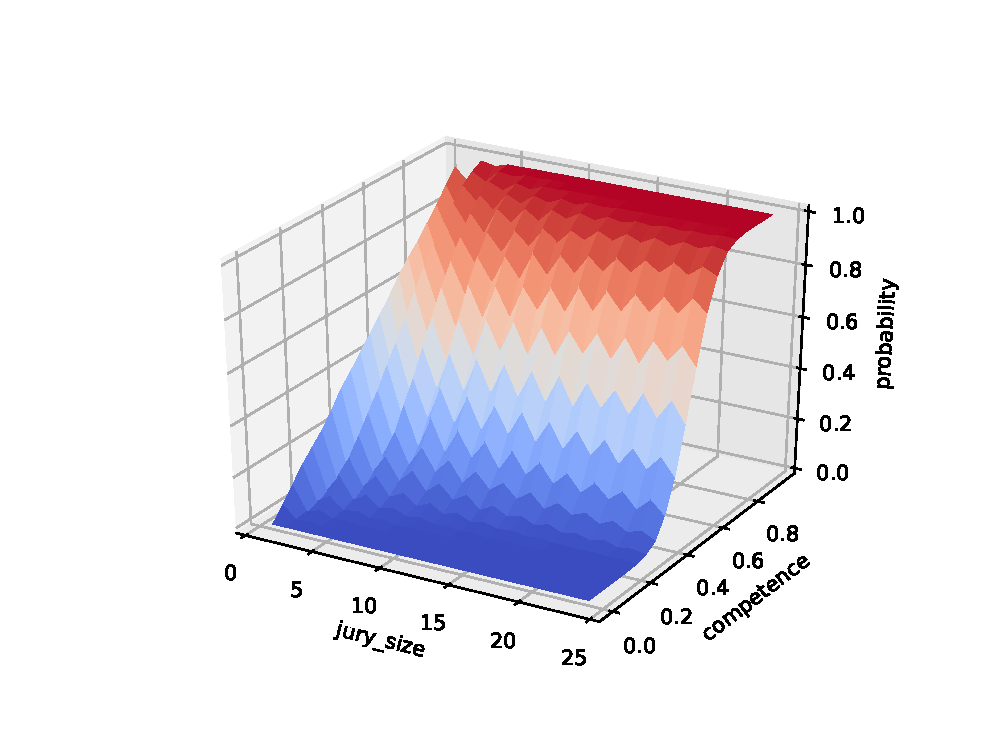
\includegraphics[width=0.75\textwidth]{images/surfplot_probs.eps}
	\caption{Surfplot of the probabilities as a function of the jury size $c$ and competence $p$.}
	\label{fig:surf_probs}
\end{figure}

\subsection{}
The probabilities for making the correct decision for the groups are:
\begin{itemize}
	\item \textbf{radiologists}: $0.850$
	\item \textbf{doctors}: $0.896$
	\item \textbf{students}: $0.826$
\end{itemize}
To reach the same probability for making the correct decision as the group of doctors, using only students. You would need 28 students. These would, collectively, have a probability of making the correct decision of $0.898$.

\section{}
The filled in table may be found below in table \ref{table:a}. Here we can see the values for different combinators.  Colors denote the choice that the classifier will make. What we can note from this table is that the choices of these classifiers are in most cases the same. 
\begin{table}[H]
	\centering
	\centering
	\begin{tabular}{ll|ll|ll|ll|ll|ll|ll}
		\multicolumn{2}{l}{$p_1(\omega|x)$} & \multicolumn{2}{l|}{$p_2(\omega|x)$} & \multicolumn{2}{l|}{$p_3(\omega|x)$} & \multicolumn{2}{l|}{Mean}                                 & \multicolumn{2}{l|}{Max}                                  & \multicolumn{2}{l|}{Min}                                  & \multicolumn{2}{l|}{Prod}                                     \\ \hline
		A                & B                & A                 & B                & A                 & B                & A                           & B                           & A                           & B                           & A                           & B                           & A                             & B                             \\ \hline
		0.9              & 0.1              & 0.9               & 0.1              & 0.0               & 1.0              & \cellcolor[HTML]{F8A102}0.6 & 0.4                         & 0.9                         & \cellcolor[HTML]{F8A102}1.0 & 0.0                         & \cellcolor[HTML]{F8A102}0.1 & 0.0                           & \cellcolor[HTML]{F8A102}0.01  \\
		0.9              & 0.1              & 0.9               & 0.1              & 0.3               & 0.7              & \cellcolor[HTML]{F8A102}0.7 & 0.3                         & \cellcolor[HTML]{F8A102}0.9 & 0.7                         & \cellcolor[HTML]{F8A102}0.3 & 0.1                         & \cellcolor[HTML]{F8A102}0.243 & 0.007                         \\
		0.9              & 0.1              & 0.2               & 0.8              & 0.1               & 0.9              & 0.4                         & \cellcolor[HTML]{F8A102}0.6 & \cellcolor[HTML]{FD6864}0.9 & \cellcolor[HTML]{FD6864}0.9 & \cellcolor[HTML]{FD6864}0.1 & \cellcolor[HTML]{FD6864}0.1 & 0.018                         & \cellcolor[HTML]{F8A102}0.072 \\
		0.0              & 1.0              & 0.0               & 1.0              & 0.0               & 1.0              & 0.0                         & \cellcolor[HTML]{F8A102}1.0 & 0.0                         & \cellcolor[HTML]{F8A102}1.0 & 0.0                         & \cellcolor[HTML]{F8A102}1.0 & 0.0                           & \cellcolor[HTML]{F8A102}1.0  
	\end{tabular}
	\caption{Classifier Combination for different methods. Values indicated in orange denote the decision the combiner would make. Values indicated in red denote a tie, the choice here is based on the implementation.}
	\label{table:a}
\end{table}

\section{}

\section{}

\section{}

\section{}

\section*{Boosting}

\section*{1}

\section*{2}

\section*{3}

\section*{4}

\section*{5}


\end{document}